\section{Introduction}

Time-series forecasting is crucial across a wide range of domains, including climate science~\cite{tsf_example_1,tsf_example_2}, energy management~\cite{tsf_example_3,tsf_example_4}, public health~\cite{tsf_example_5,tsf_example_6}, and transportation~\cite{tsf_example_7}. Datasets originating from different domains exhibit fundamentally distinct temporal dynamics, such as varying periodicity, long-term trends, irregular fluctuations, and high levels of noise. Consequently, it is essential to design forecasting model architectures that are specifically tailored to the characteristics of the data.

Most existing forecasting approaches either ``apply'' a fixed model or ``select'' from a fixed set of candidate architectures. Traditional deep learning models~\cite{DLinear,SparseTSF,PatchTST} and recent foundation models~\cite{Sundial,TimesFM,Moirai} are built with different degrees of prior knowledge and often struggle to adapt to out-of-distribution data. Given the generalization abilities of large language models (LLMs), a growing number of research has leveraged LLMs for time-series forecasting. Some work employs LLMs as forecasters by converting numerical sequences to textual representations~\cite{LLM_forecaster,GPT4MTS,TimeLLM,AutoTimes}. However, LLMs are not designed for time-series problems, which hinders their performance. Some other work utilizes LLMs as orchestrators in agent systems~\cite{TimeSeriesScientist,TimeCopilot}. These agent systems can match architectures with data characteristics to some extent. Nevertheless, without creation of novel architectures, their capacity on unseen datasets remains constrained.

Recent advances in LLM-driven coding agents highlight the possibility to ``create'' architectures using task-specific prompts. Compared to neural architecture search~\cite{nas_survey}, which relies on carefully designed search spaces and optimization strategies, coding agents can produce architectures with interpretable descriptions and requires less expert knowledge. In time-series forecasting, pioneering work~\cite{SEA-TS} utilizes tree search to guide the traversal for architecture generation. This approach biases the LLM toward optimizing a narrow subset of model classes, leading to a loss of diversity and subsequently increasing overfitting risk.

To address these limitations, we propose the Self-Evolving Time-Series Agent (\textbf{SE-TSA}), an LLM-driven programmatic evolution system to create forecasting architectures.

SE-TSA employs an iterative evolutionary loop to construct a dataset-specific forecasting model library. First, SE-TSA adopts an EXPLORE/EXPLOIT dual-strategy generation mechanism that incorporates statistical characteristics of the target domain to create forecasting architectures. Second, these architectures will be evaluated and integrated with MAP-Elites~\cite{MAP_Elites}. MAP-Elites is a quality-diversity (QD) optimization algorithm that maintains high-performing forecasters across diverse behavioral regions, thereby mitigating premature convergence. To minimize manually imposed prior knowledge, these regions are defined using a coarse categorization of existing forecasting models. Third, SE-TSA introduces a reflection mechanism that summarizes domain-specific design principles, enabling cumulative meta-learning throughout the evolutionary process. These three stages are executed iteratively to evolve the model library.

After evolution terminates, an ensemble module aggregates the best architectures discovered both globally and within the MAP-Elites archive to produce the final forecasting results, further improving robustness and performance.

\begin{nolinenumbers}
\begin{figure}[tbp]
  \centering
  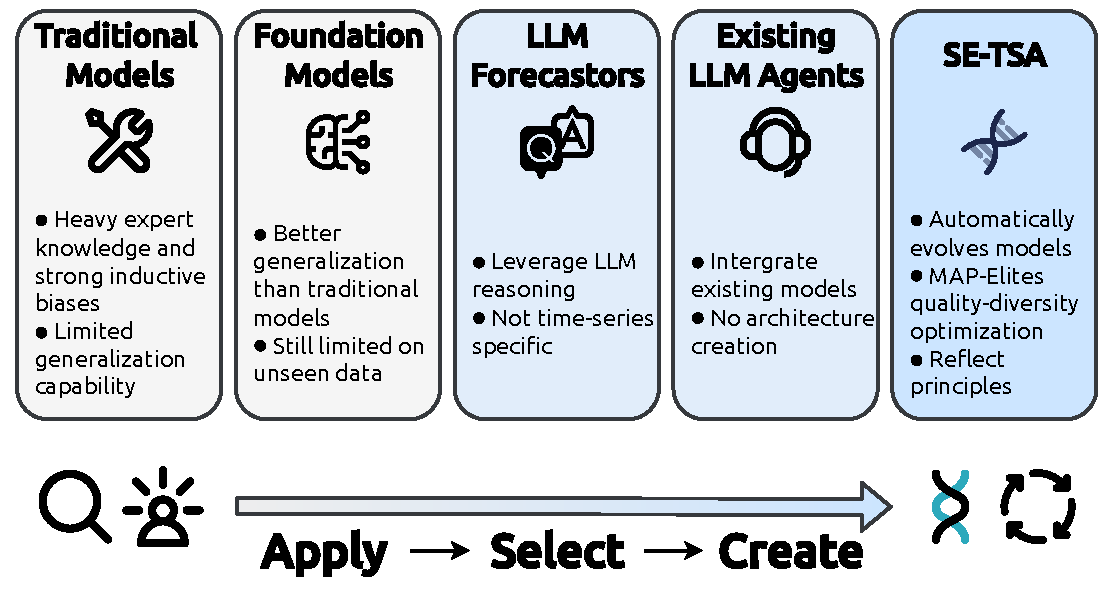
\includegraphics[width=\columnwidth]{figures/Comparison.pdf}
  \caption{Comparison between SE-TSA and existing time-series forecasting approaches.}
  \label{fig:comparison}
\end{figure}
\end{nolinenumbers}

We compare SE-TSA with other approaches as illustrated in Figure~\ref{fig:comparison}. The contributions of our proposed SE-TSA are summarized as follows:

\begin{enumerate}
  \item We propose SE-TSA, an LLM-driven evolution agent to create time-series forecasting architectures, which integrates an EXPLORE/EXPLOIT dual-strategy with MAP-Elites quality-diversity optimization.

  \item We introduce a reflection-based principle accumulation mechanism that enables interpretable meta-learning by summarizing architectural design principles in textual form.

  \item We conduct extensive experiments on nine cross-domain datasets against ten diverse baselines. Experimental results demonstrate that SE-TSA achieves superior performance on most datasets. Additional cross-domain transfer and ablation studies further validate the effectiveness of the proposed modules.
\end{enumerate}